\hypertarget{a00808}{}\section{Sidechain Inputs}
\label{a00808}\index{Sidechain Inputs@{Sidechain Inputs}}
Routing custom audio streams to a plug-\/in. 

\hypertarget{a00808_additionalFeatures_Sidechain_overview}{}\subsection{Overview of Sidechain Inputs}\label{a00808_additionalFeatures_Sidechain_overview}
If applicable, plug-\/ins may choose to enable sidechain inputs. If a sidechain is enabled, a menu is added to the plug-\/in\textquotesingle{}s header that allows the user to choose an interface or bus as the sidechain, or \char`\"{}key input\char`\"{}. Once enabled, the plug-\/in will be able to access sidechain input just like any other input signal. Currently, D\+AE is limited to mono sidechain inputs.\hypertarget{a00808_additionalFeatures_Sidechain_adding}{}\subsection{Adding a Sidechain Input to an Effect}\label{a00808_additionalFeatures_Sidechain_adding}
Setting up a sidechain input is fairly straight forward. You will want to add a physical address within your context structure, and then \char`\"{}describe\char`\"{} the sidechain in Describe.

Context Structure\+:


\begin{DoxyCode}{0}
\DoxyCodeLine{\textcolor{comment}{//=============================}}
\DoxyCodeLine{\textcolor{comment}{// Component context definitions}}
\DoxyCodeLine{\textcolor{comment}{//=============================}}
\DoxyCodeLine{}
\DoxyCodeLine{\textcolor{comment}{// Context structure}}
\DoxyCodeLine{\textcolor{keyword}{struct }SMyPlugIn\_Alg\_Context}
\DoxyCodeLine{\{}
\DoxyCodeLine{   [...]}
\DoxyCodeLine{   int32\_t  * mSideChainP;}
\DoxyCodeLine{   [...]}
\DoxyCodeLine{\};}
\DoxyCodeLine{}
\DoxyCodeLine{\textcolor{comment}{// Physical addresses within the context}}
\DoxyCodeLine{\textcolor{keyword}{enum} EDemoDist\_Alg\_PortID}
\DoxyCodeLine{\{}
\DoxyCodeLine{    [...]}
\DoxyCodeLine{    ,MyPlugIn\_AlgFieldID\_SideChain  = \mbox{\hyperlink{a00392_acf807247ecd6e5899dc9dc31644e9a1d}{AAX\_FIELD\_INDEX}} (SDemoDist\_Alg\_Context, mSideChainP)}
\DoxyCodeLine{    [...]}
\DoxyCodeLine{\};}
\end{DoxyCode}


Describe\+: 
\begin{DoxyCode}{0}
\DoxyCodeLine{\textcolor{comment}{// ***************************************************************************}}
\DoxyCodeLine{\textcolor{comment}{// ROUTINE: DescribeAlgorithmComponent}}
\DoxyCodeLine{\textcolor{comment}{// Algorithm component description}}
\DoxyCodeLine{\textcolor{comment}{// ***************************************************************************}}
\DoxyCodeLine{\textcolor{keyword}{static} \textcolor{keywordtype}{void} DescribeAlgorithmComponent( \mbox{\hyperlink{a01781}{AAX\_IComponentDescriptor}} * outDesc )}
\DoxyCodeLine{\{}
\DoxyCodeLine{    \mbox{\hyperlink{a00392_a4d8f69a697df7f70c3a8e9b8ee130d2f}{AAX\_Result}}                    err = \mbox{\hyperlink{a00494_a5f8c7439f3a706c4f8315a9609811937aeddbd1bb67e3a66e6af54a4b4a7a57b3}{AAX\_SUCCESS}};}
\DoxyCodeLine{}
\DoxyCodeLine{    [...]}
\DoxyCodeLine{    err = outDesc.\mbox{\hyperlink{a01781_a1e0c9508d1eb0c9a60a87a0fb69f1dbe}{AddSideChainIn}}(eDemoDist\_AlgFieldID\_SideChain);}
\DoxyCodeLine{    [...]}
\DoxyCodeLine{    properties->\mbox{\hyperlink{a01869_a0997671afce9a2367662c764c1d055dd}{AddProperty}} ( \mbox{\hyperlink{a00662_a13e384f22825afd3db6d68395b79ce0da3399fcd8ff459de1e3de0c98d40a5094}{AAX\_eProperty\_SupportsSideChainInput}}, \textcolor{keyword}{true} );}
\DoxyCodeLine{    [...]}
\DoxyCodeLine{\}}
\end{DoxyCode}


\begin{DoxyRefDesc}{Todo}
\item[\mbox{\hyperlink{a00785__todo000001}{Todo}}]Is properties-\/$>$Add\+Property ( A\+A\+X\+\_\+e\+Property\+\_\+\+Supports\+Side\+Chain\+Input, true ) even necessary?!?! I believe I saw a p.\+i. that does not declare this...\end{DoxyRefDesc}


In order to tell whether there is sidechain information available to your plug-\/in, check for a null pointer within your algorithm\textquotesingle{}s process function. The sidechain channel will show up as an additional stem from the original stem format you declare. That is to stay, for a stereo plug-\/in, the sidechain channel will be the third channel passed in.


\begin{DoxyCode}{0}
\DoxyCodeLine{\textcolor{comment}{//==============================================================================}}
\DoxyCodeLine{\textcolor{comment}{// Processing function definition}}
\DoxyCodeLine{\textcolor{comment}{//==============================================================================}}
\DoxyCodeLine{}
\DoxyCodeLine{\textcolor{keywordtype}{void}}
\DoxyCodeLine{\mbox{\hyperlink{a00392_aaa22112139aa627574b1ef562f579d43}{AAX\_CALLBACK}}}
\DoxyCodeLine{MyPlugIn\_AlgorithmProcessFunction (}
\DoxyCodeLine{    SMyPlugIn\_Alg\_Context * \textcolor{keyword}{const}   inInstancesBegin [],}
\DoxyCodeLine{    \textcolor{keyword}{const} \textcolor{keywordtype}{void} *                    inInstancesEnd)}
\DoxyCodeLine{\{}
\DoxyCodeLine{    [...]}
\DoxyCodeLine{    int32\_t sideChainChannel = *instance->mSideChainP;   }
\DoxyCodeLine{    \textcolor{keywordtype}{float} * AAX\_RESTRICT sideChainInput = 0;}
\DoxyCodeLine{    \textcolor{keywordflow}{if} ( sideChainChannel )}
\DoxyCodeLine{      sideChainInput = instance->mInputPP [sideChain]Channel;}
\DoxyCodeLine{    [...]}
\DoxyCodeLine{\}}
\end{DoxyCode}
 Collaboration diagram for Sidechain Inputs\+:
\nopagebreak
\begin{figure}[H]
\begin{center}
\leavevmode
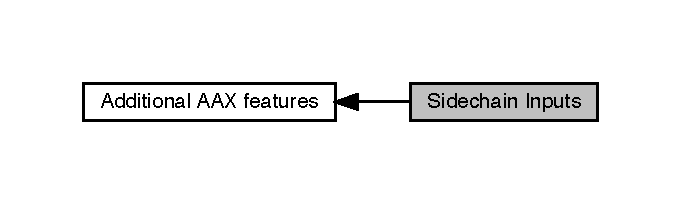
\includegraphics[width=327pt]{a00808}
\end{center}
\end{figure}
